
\section{Sprint 2}
\subsection{Introduction}
This sprint focused on developing key features for the Patient role in MindCareAI.
It included mood tracking, journaling, group messaging, social feeds, and basic chatbot support.
Patient profiles, notifications, and user preferences were also implemented.
These features aim to enhance mental health support and user engagement.

\subsection{Sprint Backlog}
\begin{table}[H] % Changed to [H] with float package for strict placement
\centering
\begin{tabular}{|p{4.2cm}|p{7.2cm}|p{2.2cm}|}
\hline
\textbf{User Story} & \textbf{Task} & \textbf{Priorities} \\
\hline
As a user, I want my role to be assigned automatically & Implement automatic patient role assignment during registration & Low \\
\hline
As a patient, I want to manage my profile information & Create patient profile model (name, phone, blood type, gender, emergency contact) & Medium \\
\hline
As a patient, I want to upload my profile picture & Add profile picture upload functionality to profile & Low \\
\hline
As a patient, I want to track my mood daily & Implement mood logging system (1--10 scale) & High \\
\hline
As a patient, I want to log my energy levels & Add energy tracking (1--5 scale) to mood logs & High \\
\hline
As a patient, I want to link moods with activities & Add activity association to mood logs & Medium \\
\hline
As a patient, I want to view my mood trends & Display 30-day mood history and statistics & High \\
\hline
As a patient, I want to write journals & Create journaling system with content, mood, weather, activity & High \\
\hline
As a patient, I want to categorize my journal entries & Add custom categories with colors and icons & Low \\
\hline
As a patient, I want to join and leave group chats & Implement join/leave support groups & Medium \\
\hline
As a patient, I want to send group messages with media & Enable text messages (5000 chars) and media upload (images, videos, PDFs) via WebSocket & Medium \\
\hline
As a patient, I want real-time feedback in chat & Add typing indicators and read receipts (WebSocket) & Medium \\
\hline
As a patient, I want to react to and search messages & Implement message reactions and search feature & Low \\
\hline
As a moderator, I want to manage group chats & Add moderator controls (delete messages, manage users) & High \\
\hline
As a patient, I want to share posts publicly & Enable post creation with media (text, image, video) & High \\
\hline
As a patient, I want to interact on the social feed & Add likes, comments, and nested replies & Medium \\
\hline
As a patient, I want timely notifications & Implement journal, mood, message, and feed notifications (WebSocket \& email) & High \\
\hline
As a patient, I want to configure my preferences & Build display settings (dark mode, language) and notification controls & Medium \\
\hline
As a patient, I want to chat with an AI & Integrate Gemini API for basic AI chatbot responses & Medium \\
\hline
\end{tabular}
\caption{Sprint 2 Backlog -- Patient Role Features}
\end{table}


\subsubsection{Functional Analysis}
\begin{figure}[H]
    \centering
    \includegraphics[width=0.9\textwidth]{images/Chapter 4/sprint2.drawio.png}
    \caption{Sprint 2 - Use Case Diagram for Sprint 2}
    \label{fig:use_case_patient}
\end{figure}

\begin{longtable}{|p{3cm}|p{12cm}|}
\hline
\textbf{Field} & \textbf{Details} \\
\hline
Title & User Roles and Profile Management \\
\hline
Actor & Patient, System \\
\hline
Description & System automatically assigns patient role during registration and enables comprehensive profile management including personal information and profile picture \\
\hline
Condition & User must complete registration process and be authenticated \\
\hline
Output & Patient role assignment, complete profile with personal details, uploaded profile picture \\
\hline
Scenario & 1. User completes registration form \newline 2. System automatically assigns patient role \newline 3. Patient accesses profile section \newline 4. Patient enters personal information (name, phone, blood type, gender, emergency contact) \newline 5. Patient uploads profile picture \newline 6. System validates and saves all profile data \\
\hline
Error handling & Registration failures, invalid profile data, profile picture upload errors, file format validation, database storage issues \\
\hline
\caption{User Roles and Profile Management Use Case}
\end{longtable}

\begin{longtable}{|p{3cm}|p{12cm}|}
\hline
\textbf{Field} & \textbf{Details} \\
\hline
Title & Mood Tracking System \\
\hline
Actor & Patient, System \\
\hline
Description & Patient logs daily mood and energy levels, associates activities, and views comprehensive mood history with trends and statistics \\
\hline
Condition & Patient must be authenticated and have active profile \\
\hline
Output & Daily mood logs, energy tracking data, activity associations, 30-day trend visualization, summary statistics \\
\hline
Scenario & 1. Patient accesses mood tracking interface \newline 2. Patient rates current mood (1-10 scale) \newline 3. Patient enters energy level (1-5 scale) \newline 4. Patient selects associated activities \newline 5. System saves mood entry with timestamp \newline 6. Patient views 30-day mood history and trends \newline 7. System displays summary statistics and patterns \\
\hline
Error handling & Invalid mood/energy values, activity selection errors, data visualization issues, historical data retrieval problems \\
\hline
\caption{Mood Tracking System Use Case}
\end{longtable}

\begin{longtable}{|p{3cm}|p{12cm}|}
\hline
\textbf{Field} & \textbf{Details} \\
\hline
Title & Journaling System \\
\hline
Actor & Patient, System \\
\hline
Description & Patient creates detailed journal entries with content, mood, weather, activities and organizes them using custom categories with colors and icons \\
\hline
Condition & Patient must be logged in and have journaling access \\
\hline
Output & Journal entries with rich metadata, custom categories with visual identifiers \\
\hline
Scenario & 1. Patient opens journaling interface \newline 2. Patient writes journal content \newline 3. Patient records current general day mood and weather conditions \newline 4. Patient can w relevant activities \newline 5. Patient creates or selects custom category with color and icon \newline 6. System saves journal entry with all metadata \\
\hline
Error handling & Content validation errors, category creation failures, metadata saving issues, journal entry storage problems \\
\hline
\caption{Journaling System Use Case}
\end{longtable}

\begin{longtable}{|p{3cm}|p{12cm}|}
\hline
\textbf{Field} & \textbf{Details} \\
\hline
Title & Group Messaging Community \\
\hline
Actor & Patient, System \\
\hline
Description & Patient participates in support group messaging with real-time communication, media sharing, and moderation features using WebSocket technology \\
\hline
Condition & Patient must be authenticated and have group messaging permissions \\
\hline
Output & Real-time group messaging, media attachments, typing indicators, read receipts, message reactions, search results, moderation actions \\
\hline
Scenario & 1. Patient joins support group \newline 2. Patient sends text messages (up to 5000 characters) via WebSocket \newline 3. Patient uploads media attachments (images, videos, PDFs) \newline 4. System displays typing indicators and read receipts in real-time \newline 5. Patient reacts to messages and searches chat history \newline 6. Moderator manages inappropriate content and users \newline 7. Patient can leave group when needed \\
\hline
Error handling & WebSocket connection failures, media upload errors, message validation issues, moderation action failures, search functionality problems \\
\hline
\caption{Group Messaging Community Use Case}
\end{longtable}

\begin{longtable}{|p{3cm}|p{12cm}|}
\hline
\textbf{Field} & \textbf{Details} \\
\hline
Title & Social Feeds \\
\hline
Actor & Patient, System \\
\hline
Description & Patient creates and shares posts with media content and engages with community through likes, comments, and nested comment discussions \\
\hline
Condition & Patient must be authenticated and have social feed access \\
\hline
Output & Public posts with media content, engagement metrics (likes), comment threads with nested replies \\
\hline
Scenario & 1. Patient creates new post with text and media content \newline 2. Patient publishes post to social feed \newline 3. Patient browses community posts \newline 4. Patient likes posts and writes comments \newline 5. Patient creates nested replies to existing comments \newline 6. System tracks all engagement activities \\
\hline
Error handling & Post creation failures, media upload errors, engagement tracking issues, nested comment depth limitations, content moderation problems \\
\hline
\caption{Social Feeds Use Case}
\end{longtable}

\begin{longtable}{|p{3cm}|p{12cm}|}
\hline
\textbf{Field} & \textbf{Details} \\
\hline
Title & Notification System \\
\hline
Actor & Patient, System \\
\hline
Description & System delivers real-time notifications for journal activities, messaging alerts, mood tracking reminders, and feed engagement using WebSocket technology \\
\hline
Condition & Patient must be authenticated and have notification permissions enabled \\
\hline
Output & Real-time notifications for journal confirmations, messaging alerts, mood reminders, feed engagement notifications \\
\hline
Scenario & 1. System monitors user activities requiring notifications \newline 2. System sends journal creation confirmations \newline 3. System delivers messaging alerts (new messages, typing indicators) via WebSocket \newline 4. System sends mood tracking reminders \newline 5. System notifies about feed engagement (likes, comments) \newline 6. Patient receives notifications in real-time \\
\hline
Error handling & WebSocket delivery failures, notification timing issues, permission errors, notification queue overload \\
\hline
\caption{Notification System Use Case}
\end{longtable}

\begin{longtable}{|p{3cm}|p{12cm}|}
\hline
\textbf{Field} & \textbf{Details} \\
\hline
Title & User Preferences Management \\
\hline
Actor & Patient, System \\
\hline
Description & Patient customizes application experience through display settings and notification controls with selective notification management \\
\hline
Condition & Patient must be authenticated and have access to preferences \\
\hline
Output & Customized display settings, configured notification preferences, selective notification controls \\
\hline
Scenario & 1. Patient accesses user preferences interface \newline 2. Patient configures display settings (dark mode, language) \newline 3. Patient sets notification controls (email, in-app preferences) \newline 4. Patient selectively disables specific notification types \newline 5. System applies all preference changes \newline 6. System maintains preferences across sessions \\
\hline
Error handling & Preference saving failures, display setting application errors, notification control conflicts, session persistence issues \\
\hline
\caption{User Preferences Management Use Case}
\end{longtable}

\begin{longtable}{|p{3cm}|p{12cm}|}
\hline
\textbf{Field} & \textbf{Details} \\
\hline
Title & Basic AI Chatbot \\
\hline
Actor & Patient, System \\
\hline
Description & Patient interacts with AI-powered chatbot integrated with Gemini API for simple conversational responses and basic user interaction support \\
\hline
Condition & Patient must be authenticated and have chatbot access enabled \\
\hline
Output & AI-generated conversational responses, basic interaction support, conversation history \\
\hline
Scenario & 1. Patient accesses AI chatbot interface \newline 2. Patient sends message or question to chatbot \newline 3. System processes request through Gemini API integration \newline 4. System generates simple conversational response \newline 5. Patient continues basic user interaction \newline 6. System maintains conversation context \\
\hline
Error handling & Gemini API connection failures, response generation timeouts, inappropriate content filtering, conversation context errors \\
\hline
\caption{Basic AI Chatbot Use Case}
\end{longtable}
\newpage

\subsection{Database Design}

This subsection presents the database schema used in the system. The design ensures data integrity, scalability, and normalization.
 
\vfill
\begin{figure}[H]
    \centering
    \includegraphics[width=1\textheight, height=0.65\textwidth, angle=90]{images/Chapter 4/ed_sprint2.png}
    \caption{Database Design Diagram}
    \label{fig:database-design}
\end{figure}



\vfill
\newpage

\subsection{Software Design}

This section provides a structural and behavioral view of the software system using UML diagrams.

\paragraph{Class Diagram}

The class diagram outlines the static structure of the system, detailing the classes, attributes, methods, and relationships.

\begin{figure}[H]
    \centering
    \includegraphics[width=0.85\textwidth]{images/Chapter 4/sprint2_diagram_classe.png}
    \caption{Class Diagram of the System}
    \label{fig:class-diagram}
\end{figure}

\paragraph{Sequence Diagrams}

The following sequence diagrams illustrate the dynamic behavior of each major system component, focusing on object interactions over time for each Django application in Sprint 2.

\begin{figure}[H]
    \centering
    \includegraphics[width=0.75\textwidth]{Auth_Sequence_Diagram.png}
    \caption{Authentication \& Role Assignment Sequence Diagram}
    \label{fig:auth-sequence-diagram}
\end{figure}

\begin{figure}[H]
    \centering
    \includegraphics[width=0.75\textwidth]{Patient_Sequence_Diagram.png}
    \caption{Patient Profile Management Sequence Diagram}
    \label{fig:patient-sequence-diagram}
\end{figure}

\begin{figure}[H]
    \centering
    \includegraphics[width=0.75\textwidth]{Mood_Sequence_Diagram.png}
    \caption{Mood Tracking \& Journaling System Sequence Diagram}
    \label{fig:mood-sequence-diagram}
\end{figure}

\begin{figure}[H]
    \centering
    \includegraphics[width=0.75\textwidth]{Messaging_Sequence_Diagram.png}
    \caption{Group Messaging System Sequence Diagram}
    \label{fig:messaging-sequence-diagram}
\end{figure}

\begin{figure}[H]
    \centering
    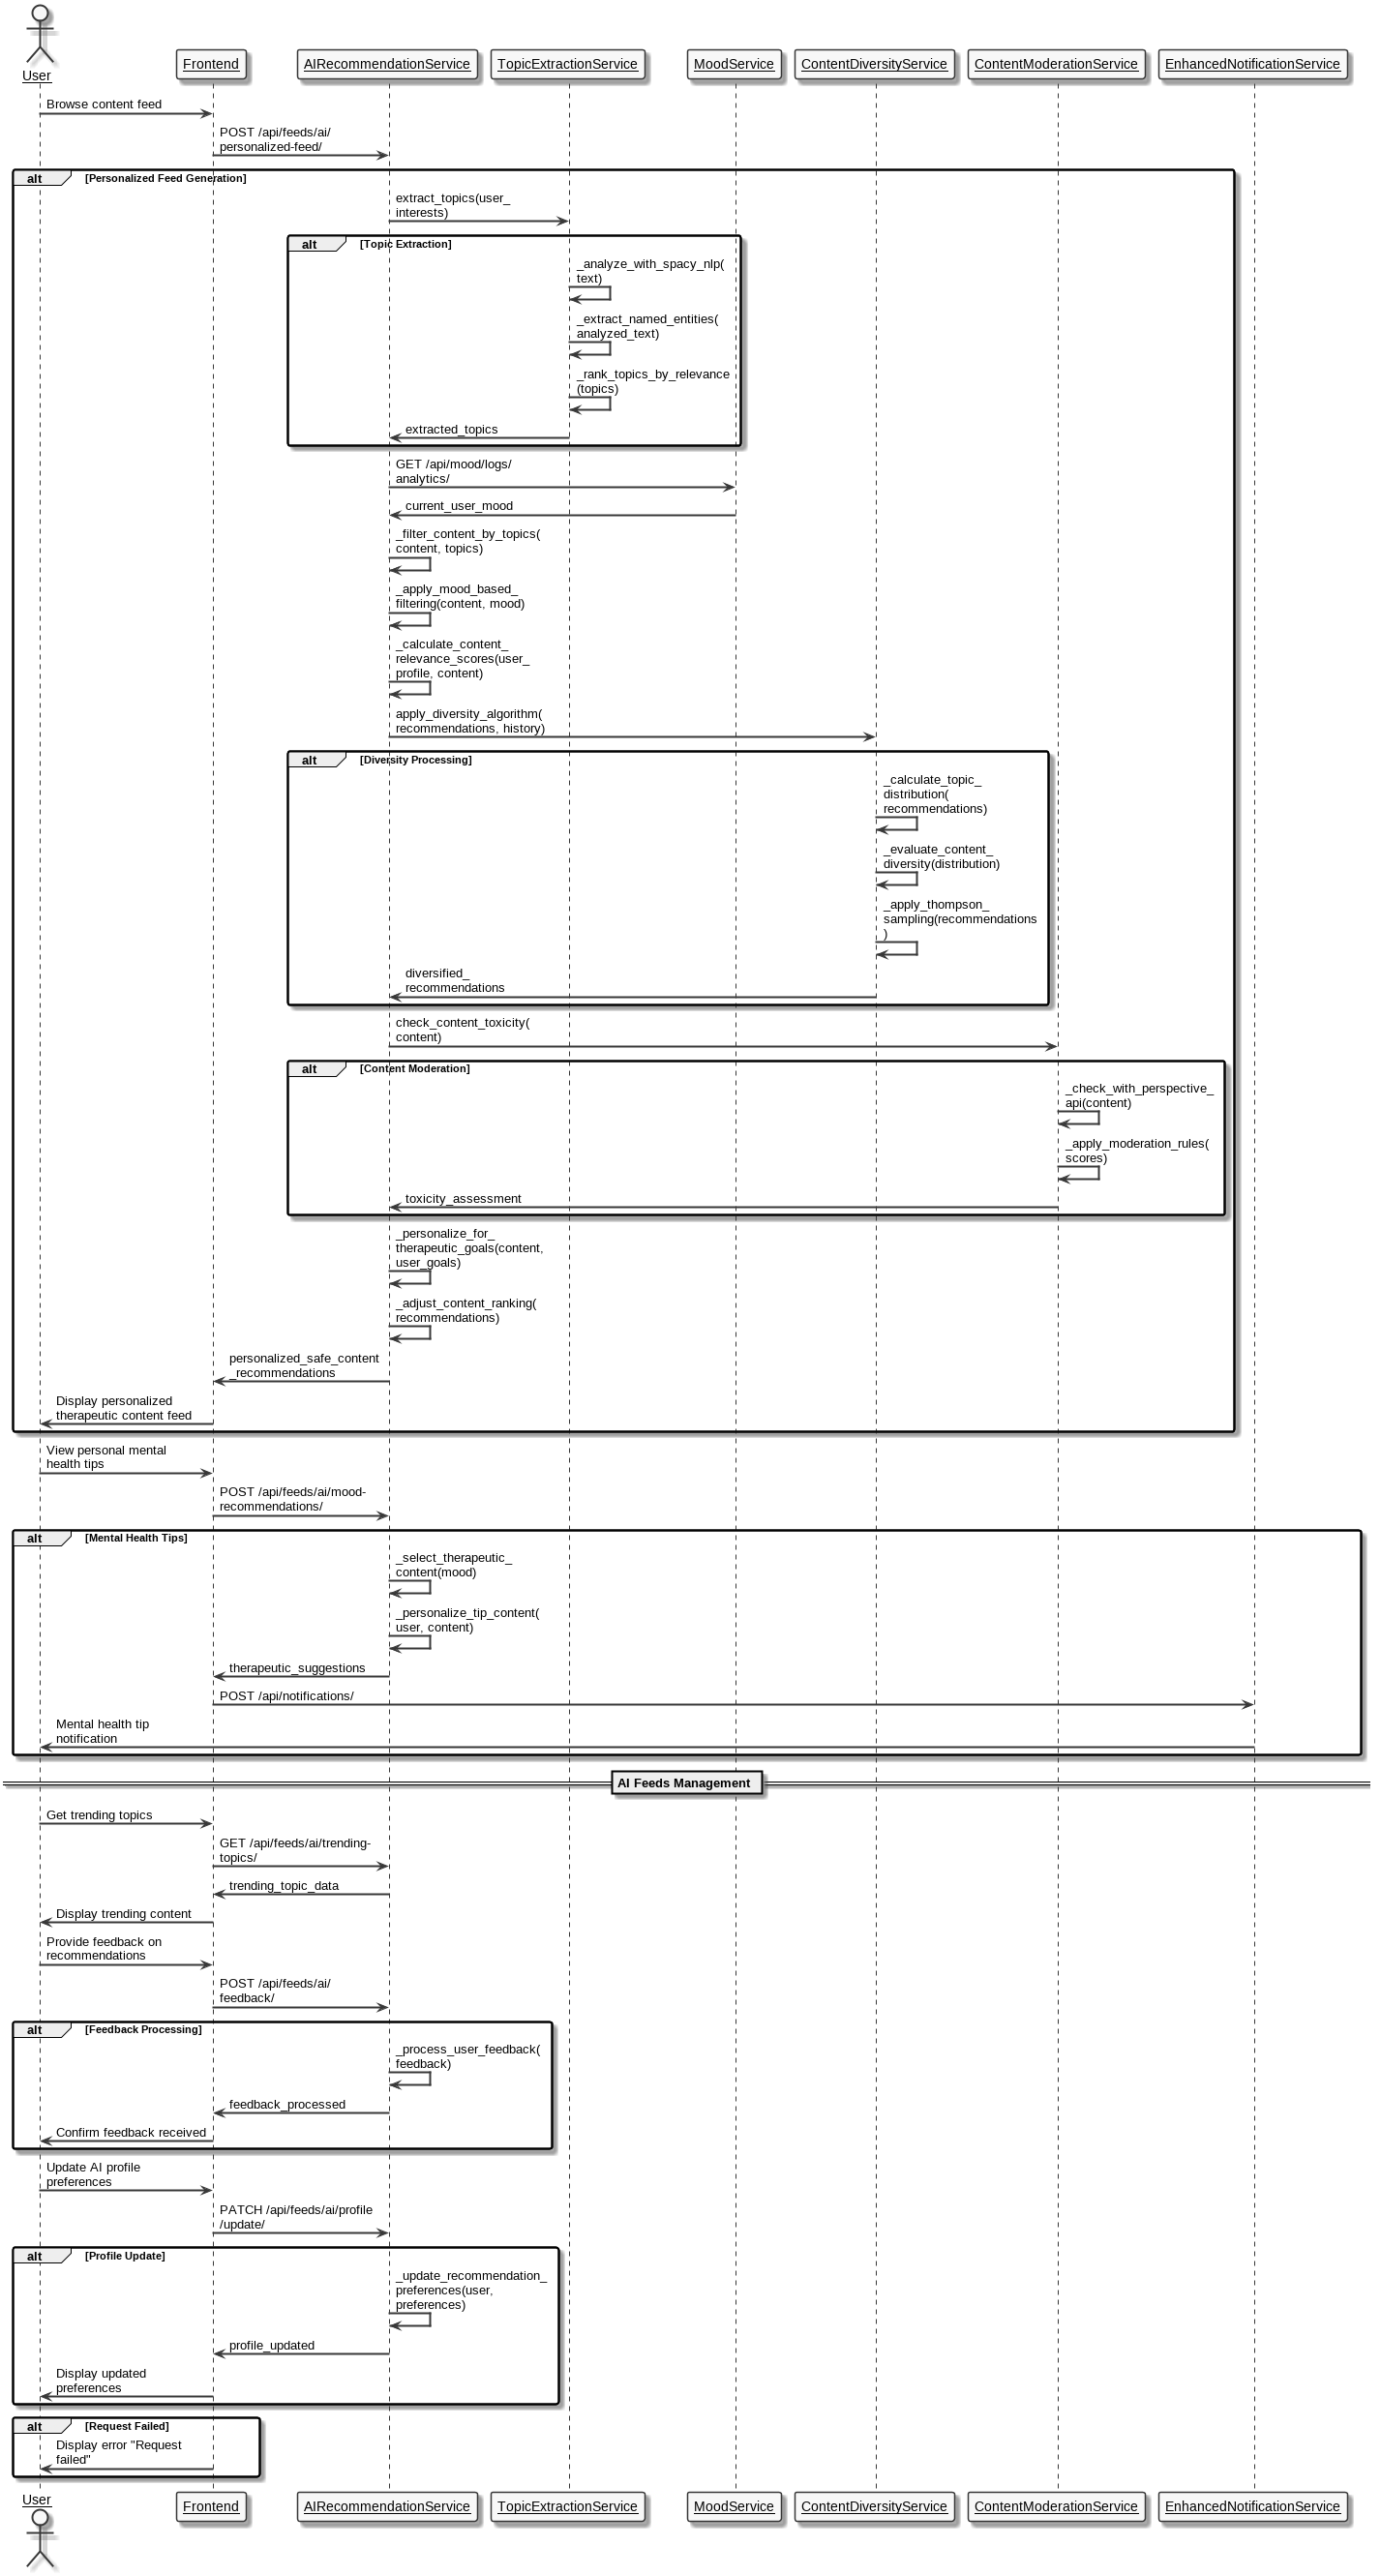
\includegraphics[width=0.75\textwidth]{Feeds_Sequence_Diagram.png}
    \caption{Social Feed System Sequence Diagram}
    \label{fig:feeds-sequence-diagram}
\end{figure}

\begin{figure}[H]
    \centering
    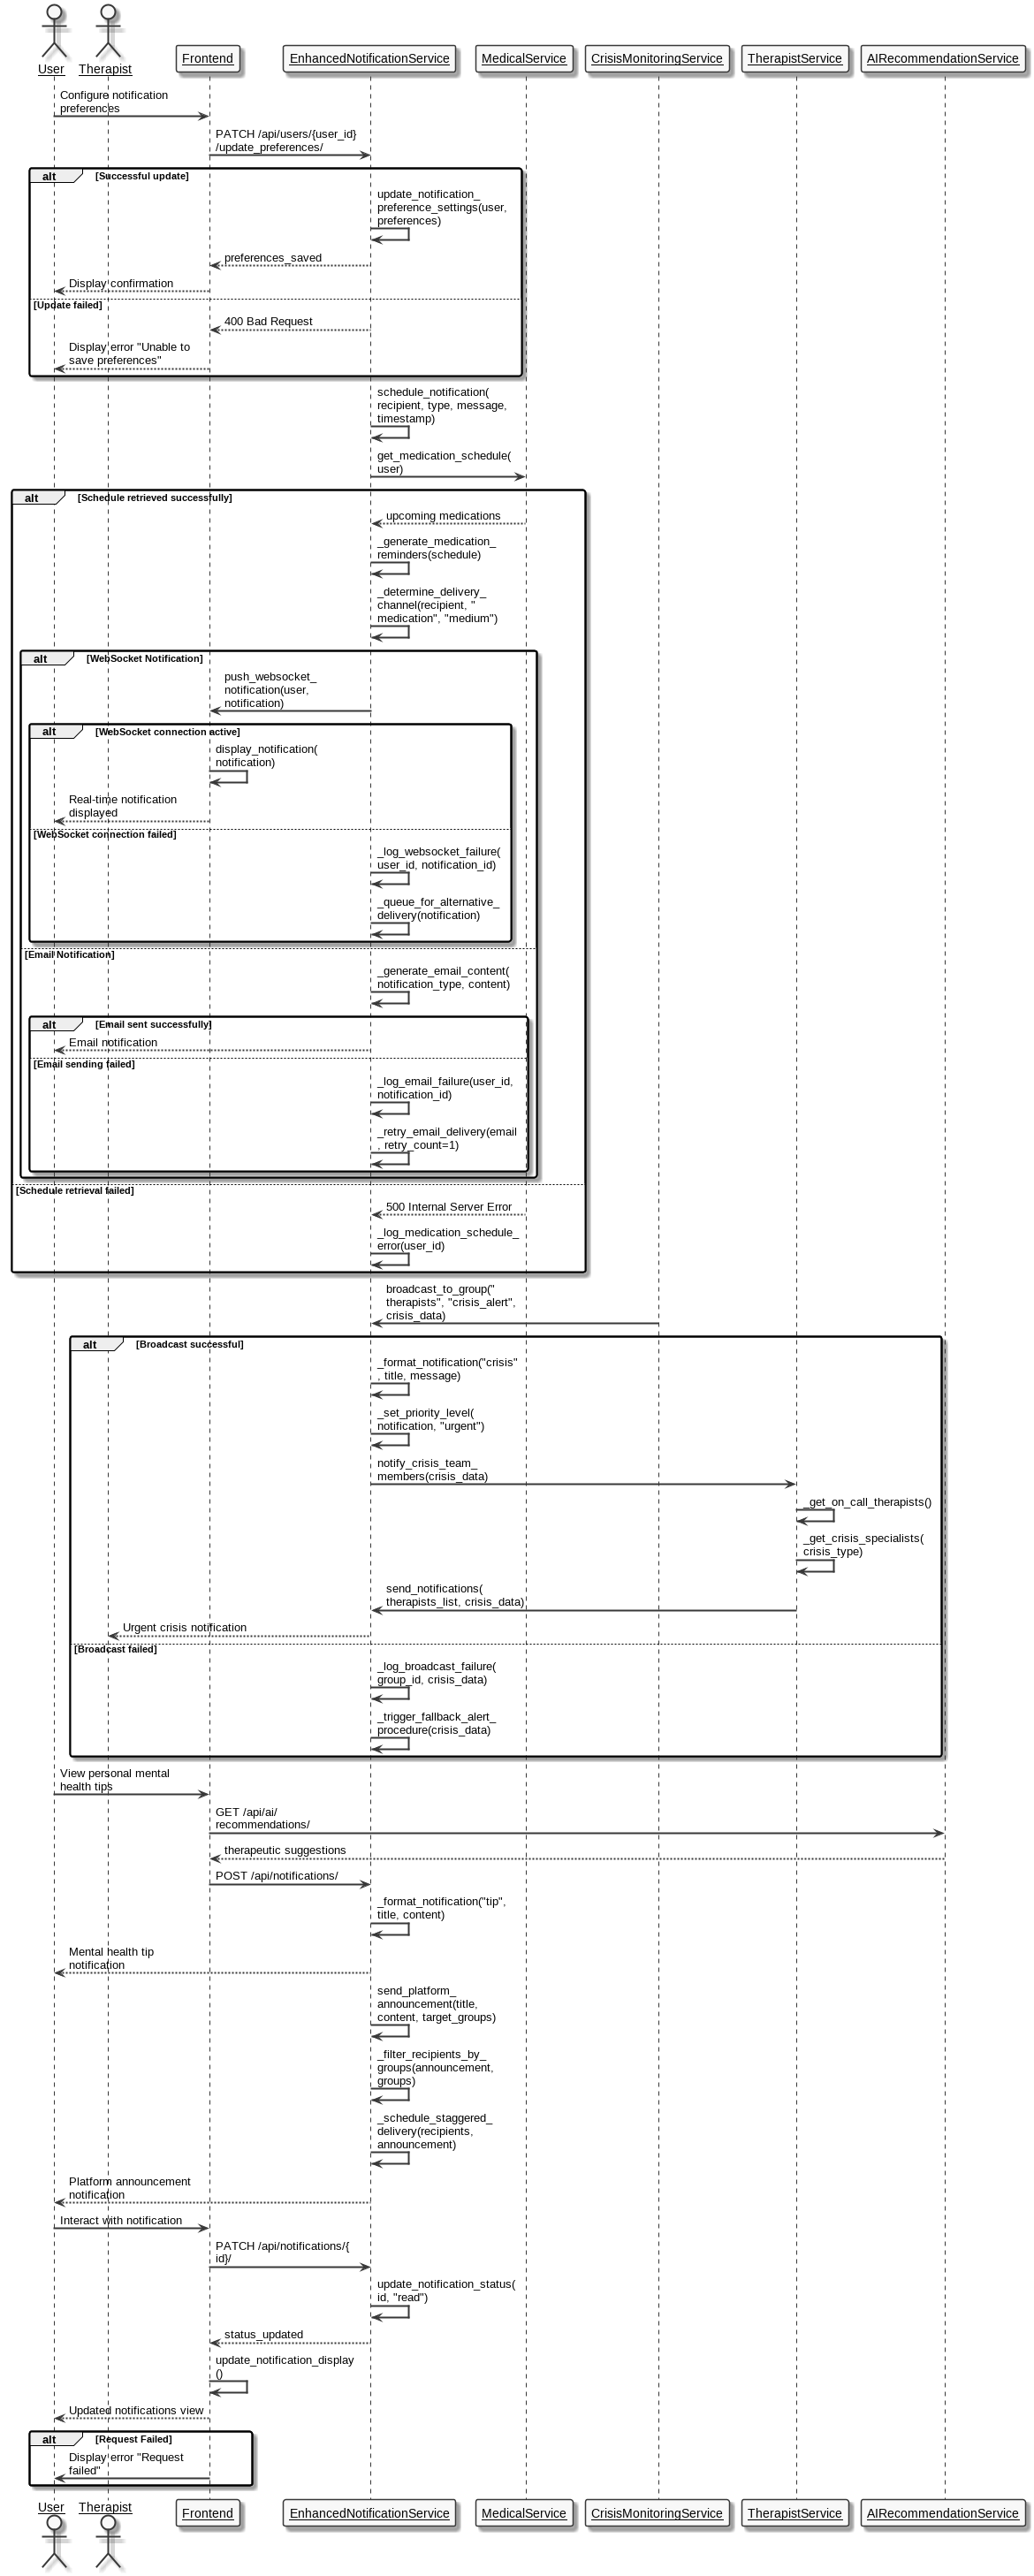
\includegraphics[width=0.75\textwidth]{Notifications_Sequence_Diagram.png}
    \caption{Notification System Sequence Diagram}
    \label{fig:notifications-sequence-diagram}
\end{figure}

\begin{figure}[H]
    \centering
    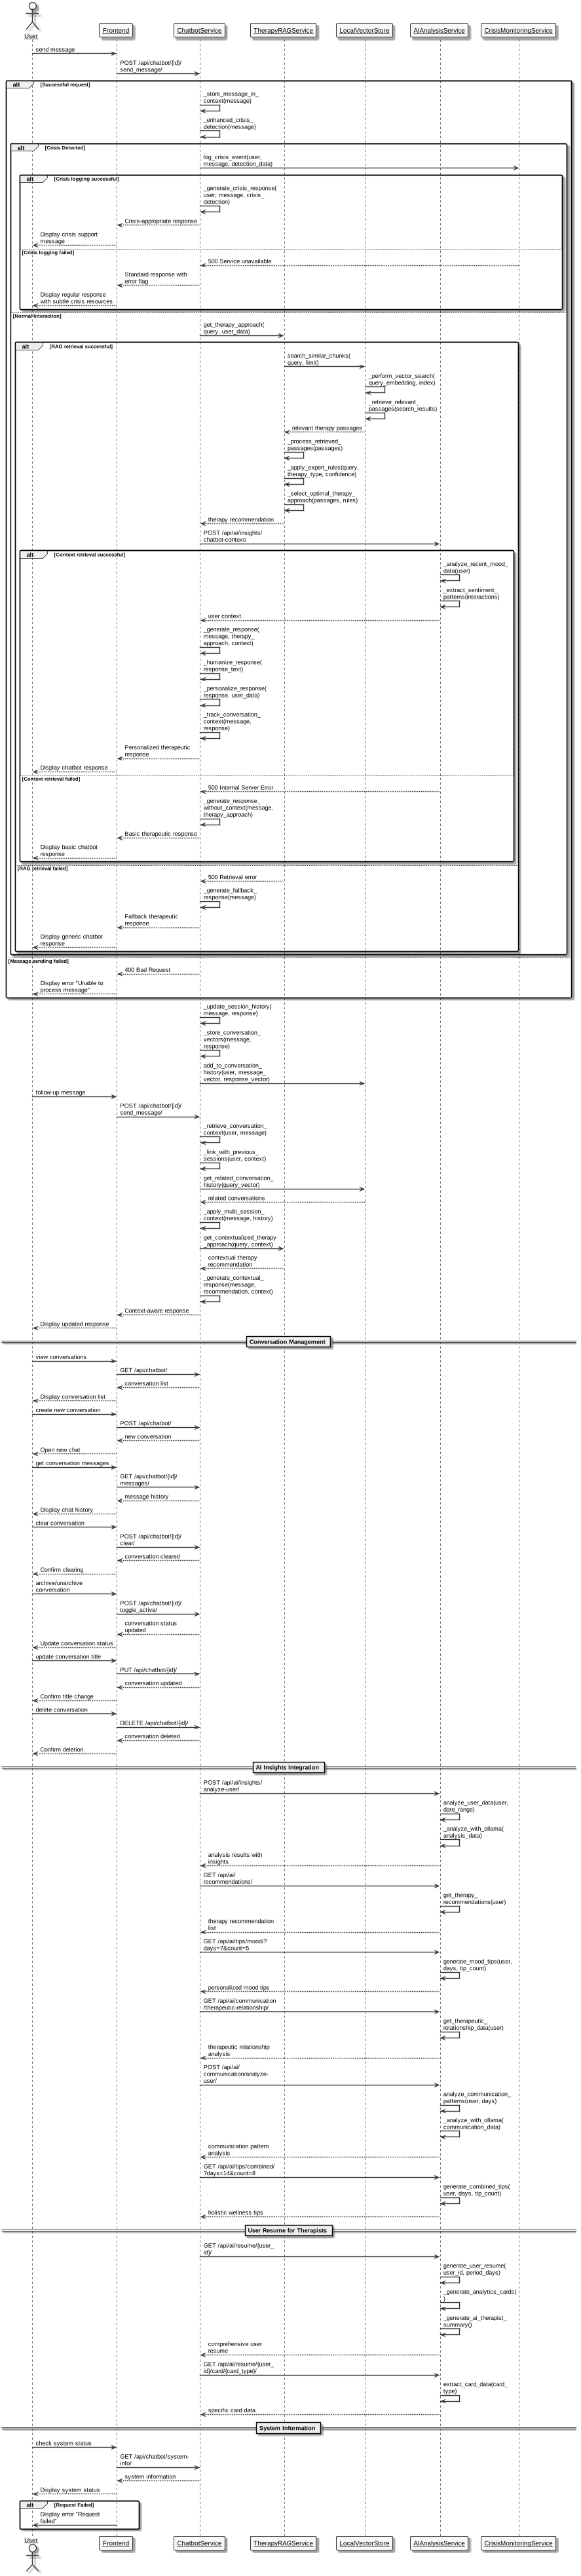
\includegraphics[width=0.75\textwidth]{Chatbot_Sequence_Diagram.png}
    \caption{AI Chatbot System Sequence Diagram}
    \label{fig:chatbot-sequence-diagram}
\end{figure}